\section{Human Evaluations on \bcp{}}
\label{secs:appendix_bcp_evals}


\subsection{Effect of Model Scale}
\begin{figure}[t]
    \centering
    \footnotesize
    \setlength\tabcolsep{2pt}
    \begin{tabular}{>{\centering\arraybackslash}p{0.5\textwidth}>{\centering\arraybackslash}p{0.5\textwidth}}
        \multicolumn{2}{c}{\textbf{Image Realism (\bdraw 20B vs. 3B model)}} \\
        \textbf{Categories} & \textbf{Challenge Aspects} \\
        \vspace{-0.1in}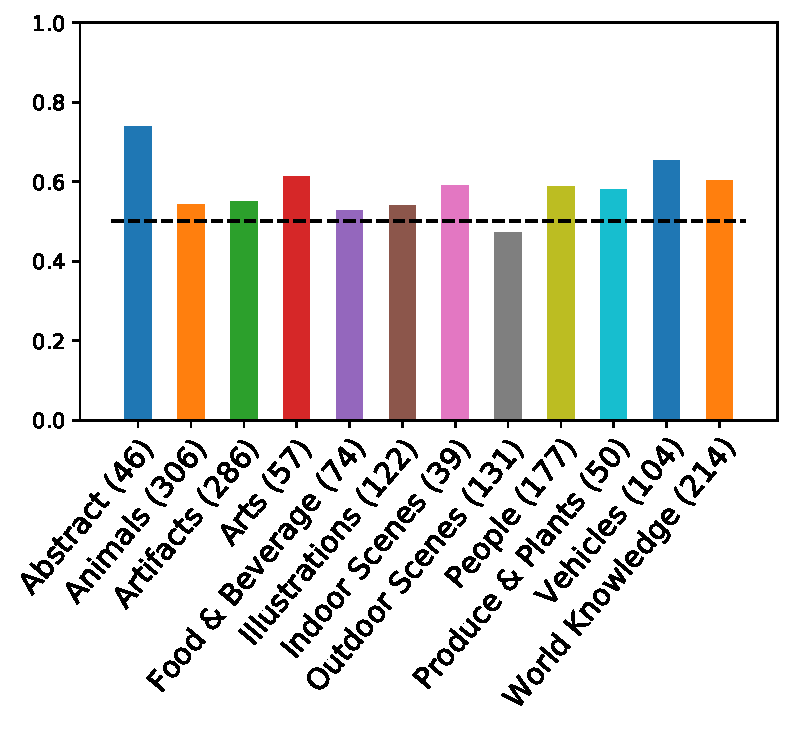
\includegraphics[width=0.48\textwidth]{figures/bcp_charts/bcp_20b_3b_breakdown_category_realism.pdf} &
        \vspace{-0.1in}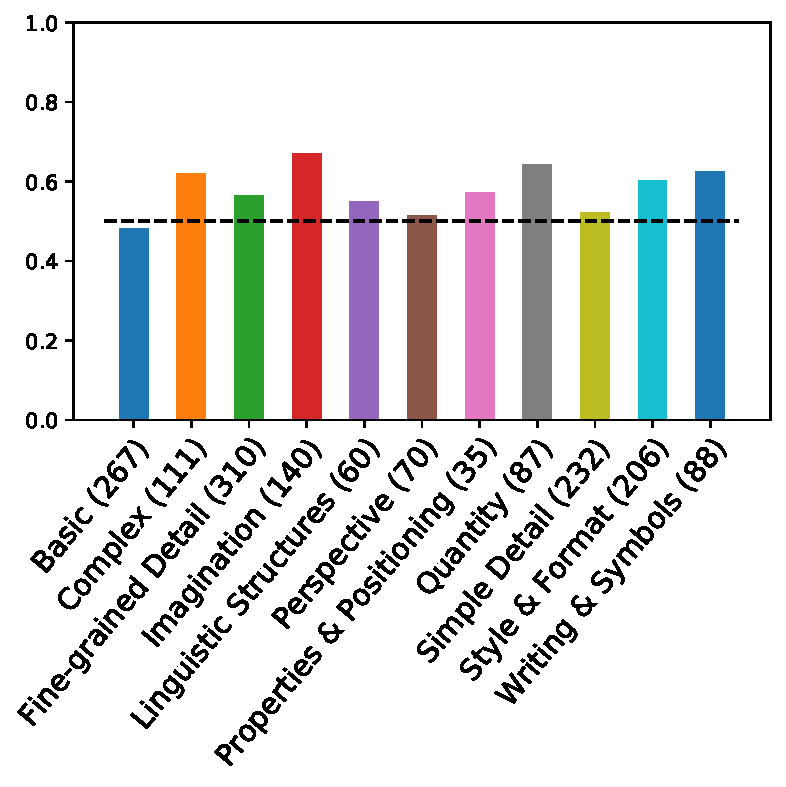
\includegraphics[width=0.48\textwidth]{figures/bcp_charts/bcp_20b_3b_breakdown_complexity_realism.pdf} \vspace{1mm} \\
    \end{tabular} 
    \caption{
    Breakdown of human preferences of the realism of images from the \bdraw 20B model over the 3B model in terms of \bcpa{} categories ({\it left}) and challenge aspects ({\it right}).}
    \label{figs:bcp_20b_3b_realism_breakdown}
\end{figure}



Figure~\ref{figs:bcp_20b_3b_realism_breakdown} further breaks down the human preferences of the 20B model (over the 3B model) across \bcpa{} categories (left) and challenge aspects (right) for image realism. 
We observe that as compared to the human preference for image-text match (Figure~\ref{figs:bcp_20b_3b_language}), the 20B model wins out on image realism by a smaller margin. 
This suggests that model scaling mostly benefits language understanding and image-text match, as compared to improvements on image realism. This makes intuitive sense: image realism is largely dependent on the quality of the ViT-VQGAN quantizer, and thus scaling the transformer model would primarily improve the ability of \bdraw to composite and represent natural language concepts. 

In terms of individual categories, the 20B model is preferred over the 3B for the majority of categories, most prominently \bcpstyle{Abstract}, \bcpstyle{World Knowledge}, \bcpstyle{Vehicles}, and \bcpstyle{Arts}. For other categories, the human preference is mostly on par for the 20B and 3B models, with the 3B model being slightly preferred for outdoor scenes. Interestingly, we observe that over the challenge aspects, the 20B model outperforms the 3B model on all challenge aspects, \textit{except} for \bcpstyle{Basic} prompts. This suggests that the 3B model scale is sufficient to handle the basic prompts in \bcp (which generally contain more simple prompts). Increasing model size to 20B does not help and may even slightly harm generation quality on these concepts. In contrast, the 20B model achieves a marked improvement in performance on more difficult \bcp prompts, such as those in the \bcpstyle{Complex} and \bcpstyle{Imagination} challenge dimensions. This aligns with our observations on the significant improvement of the 20B model on prompts from the \bcpstyle{Abstract} category.


\subsection{Comparison Against Retrieval Baseline}

\begin{figure}[t]
    \centering
    \footnotesize
    \setlength\tabcolsep{2pt}
    \begin{tabular}{>{\centering\arraybackslash}p{0.5\textwidth}>{\centering\arraybackslash}p{0.5\textwidth}}
        \multicolumn{2}{c}{\textbf{Image-Text Match (\bdraw 20B vs. Retrieval)}} \\
        \textbf{Categories} & \textbf{Challenge Aspects} \\
        \vspace{-0.1in}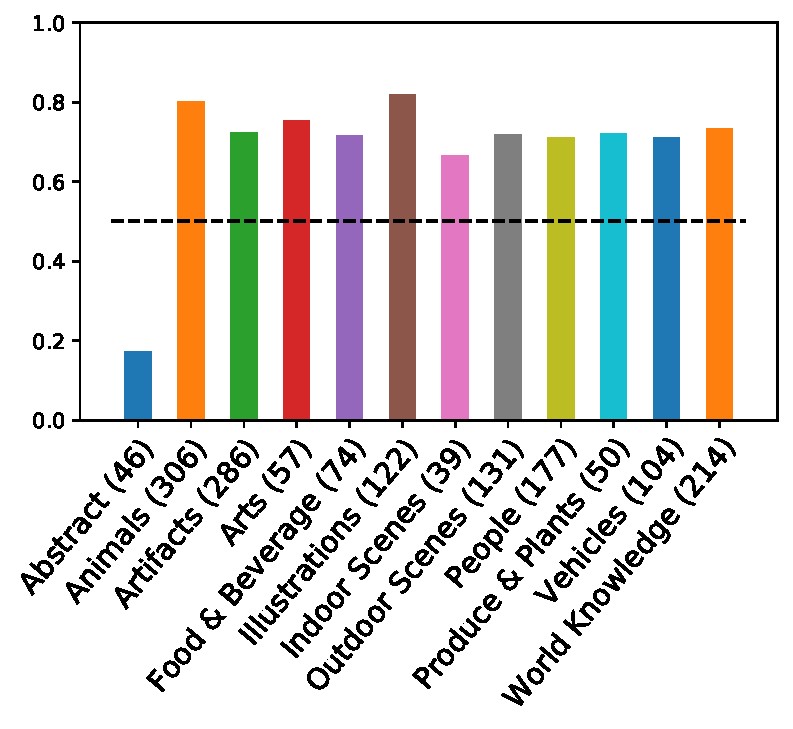
\includegraphics[width=0.48\textwidth]{figures/bcp_charts/bcp_20b_retrieval_breakdown_category_language.pdf} &
        \vspace{-0.1in}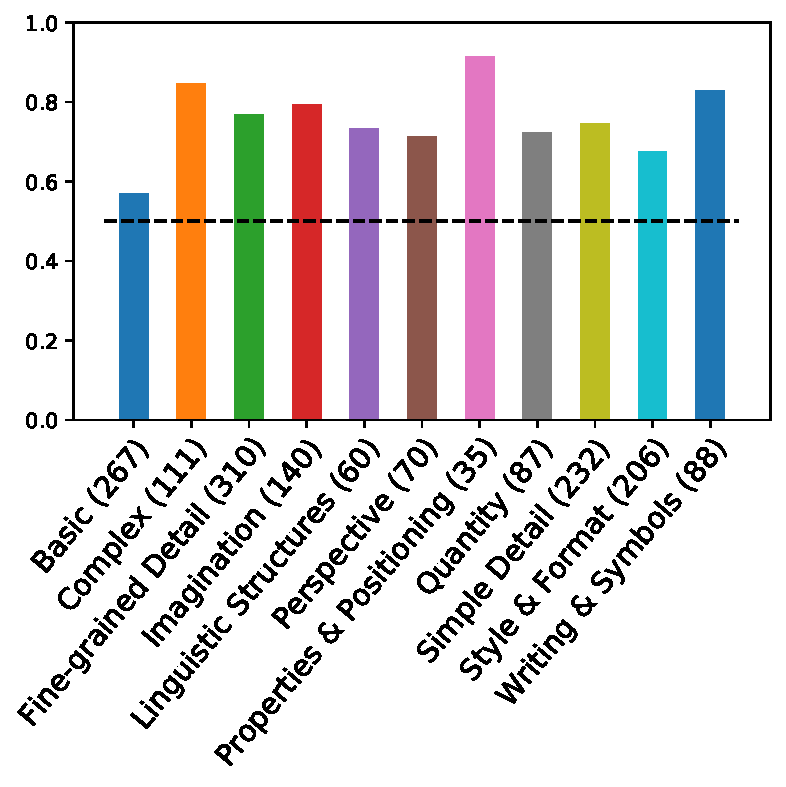
\includegraphics[width=0.48\textwidth]{figures/bcp_charts/bcp_20b_retrieval_breakdown_complexity_language.pdf} \vspace{1mm} \\
    \end{tabular} 
    \caption{
    Breakdown of human preferences of the image-text match of images from the \bdraw 20B model over the retrieval baseline in terms of \bcpa{} categories ({\it left}) and challenge aspects ({\it right}).}
    \label{figs:bcp_retrieval_lang_breakdown}
\end{figure}


\begin{figure}[t]
    \centering
    \footnotesize
    \setlength\tabcolsep{2pt}
    \begin{tabular}{>{\centering\arraybackslash}p{0.5\textwidth}>{\centering\arraybackslash}p{0.5\textwidth}}
        \multicolumn{2}{c}{\textbf{Image Realism (\bdraw 20B vs. Retrieval)}} \\
        \textbf{Categories} & \textbf{Challenge Aspects} \\
        \vspace{-0.1in}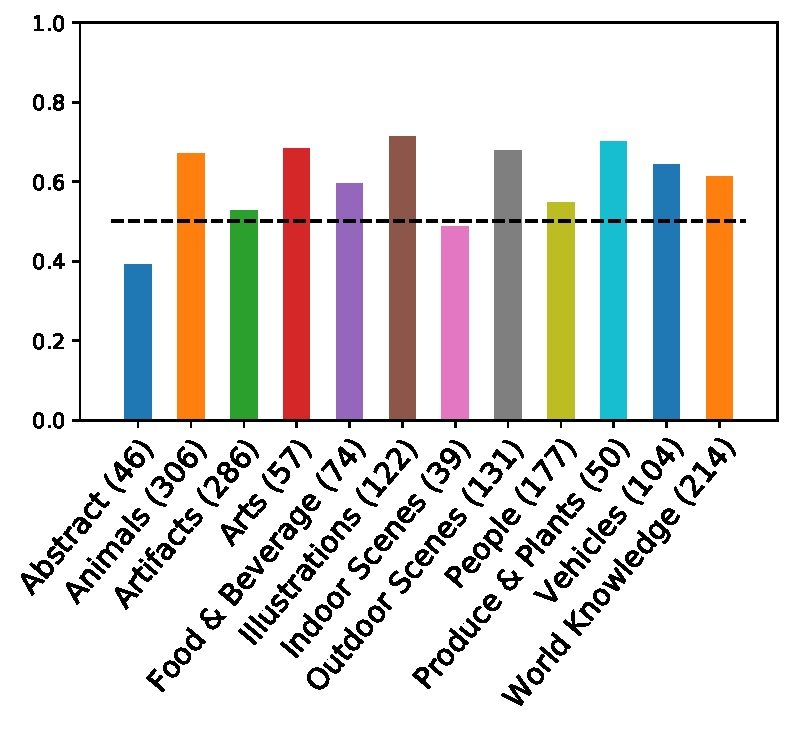
\includegraphics[width=0.48\textwidth]{figures/bcp_charts/bcp_20b_retrieval_breakdown_category_realism.pdf} &
        \vspace{-0.1in}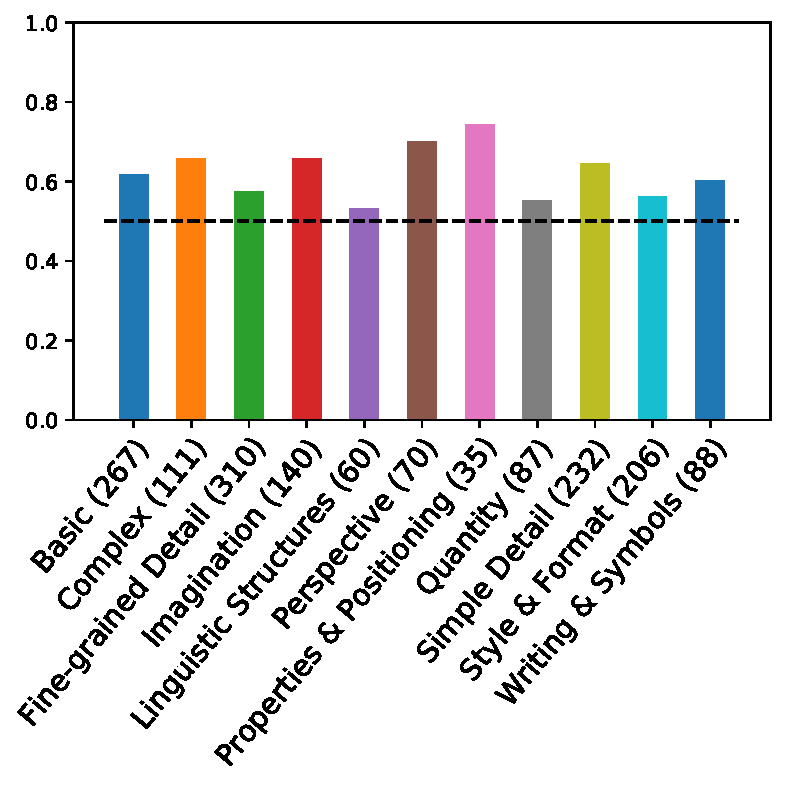
\includegraphics[width=0.48\textwidth]{figures/bcp_charts/bcp_20b_retrieval_breakdown_complexity_realism.pdf} \vspace{1mm} \\
    \end{tabular} 
    \caption{
    Breakdown of human preferences of the realism of images from the \bdraw 20B model over the retrieval baseline in terms of \bcpa{} categories ({\it left}) and challenge aspects ({\it right}).}
    \label{figs:bcp_retrieval_realism_breakdown}
\end{figure}

In addition to comparing our 20B and 3B models, we also run human evaluations of the \bdraw 20B model against the retrieval baseline. Figure~\ref{figs:bcp_retrieval_lang_breakdown} and \ref{figs:bcp_retrieval_realism_breakdown} show human preference of the 20B model (over the retrieval baseline) across \bcpa{}.
On image-text match (Figure~\ref{figs:bcp_retrieval_lang_breakdown}), the \bdraw model significantly outperforms the retrieval baseline in most categories, except for \bcpstyle{Abstract}. This highlights the difficulty in generating good images for \bcpstyle{Abstract} prompts, which may be a potential area of improvement for future work. Along different challenge aspects, \bdraw outperforms the retrieval baseline in every category on image-text match, which we attribute to the improved ability of \bdraw to synthesize images for diverse and complex prompts. Many of the harder prompts in the \bcpa{} are  `adversarial' in nature, and were designed to test the limits of text-to-image synthesis models. These prompts are generally unlikely to have appeared in standard training datasets, and consequently difficult for retrieval based models which rely on retrieving the closest match from our training corpus. The positive results along this evaluation highlight the strength of a generative model such as \bdraw, and its ability to handle diverse and creative prompts.

When evaluated on image realism (Figure~\ref{figs:bcp_retrieval_realism_breakdown}), \bdraw fares well against the retrieval baseline, and is preferred by human annotators across the majority of the \bcpa{} categories (except \bcpstyle{Abstract} and \bcpstyle{Indoor Scenes}), as well as preferred along all challenge aspect dimensions. We note that this is a remarkable feat, considering that the retrieval model retrieves \textit{real images} from a training corpus. These results highlight the ability of \bdraw to synthesize realistic images, which are deemed by human evaluators as close to photorealistic (or even more photorealistic, in some cases).